\documentclass[12pt,onecolumn]{article}
\usepackage{listings}
\usepackage{float}
\usepackage{mathtools}
\usepackage[english,russian]{babel}
\everymath{\displaystyle}
\usepackage{hyperref}
\usepackage[usenames]{color}
\usepackage{colortbl}
\usepackage{placeins}
\usepackage{xcolor}
\usepackage{verbatim}
\usepackage[T2A]{fontenc}
\usepackage{geometry}
\geometry{
  a4paper,
  top=25mm, 
  right=15mm, 
  bottom=25mm, 
  left=15mm
}

\begin{document}
\setcounter{tocdepth}{4}
\begin{center}
    Санкт-Петербургский Национальный Исследовательский\\ 
    Университет ИТМО\\
    Мегафакультет Компьютерных Технологий и Управления\\
    Факультет Программной Инженерии и Компьютерной Техники \\
    
\includegraphics[scale=0.3]{images/itm.jpg} % нужно закинуть картинку логтипа в папку с отчетом
\end{center}
\vspace{1cm}


\begin{center}
    \textbf{Лабораторная работа №3}\\
    по дисциплине\\
    \textbf{Информатика}
\end{center}

\vspace{2cm}

\begin{flushright}
  Выполнил Студент  группы number\\
  \textbf{Student's name}\\
  Преподаватель: \\
  \textbf{Teacher's name}\\
\end{flushright}

\vspace{10cm}
\begin{center}
    г. Санкт-Петербург\\
    2021г.
\end{center}
\newpage
\tableofcontents
\newpage
\begin{flushleft}
\section{Выполнение заданий}
\subsection{Задание 1}
\paragraph{Текст задания:}
\hfill \break
1) Реализуйте программный продукт на языке Python, используя регулярные выражения по варианту, представленному в таблице.\\
2) Для своей программы придумайте минимум 5 тестов. Каждый тест является отдельной сущностью, передаваемой регулярному выражению для обработки. Для каждого теста необходимо самостоятельно (без использования регулярных выражений) найти правильный ответ. После чего сравнить ответ, выданный программой, и полученный самостоятельно.\\
3) Программа должна считать количество смайликов определённого вида (вид смайлика описан в таблице вариантов) в предложенном тексте. Все смайлики имеют такую структуру: [глаза][нос][рот].\\
Вариантом является различные наборы глаз, носов и ртов.\\
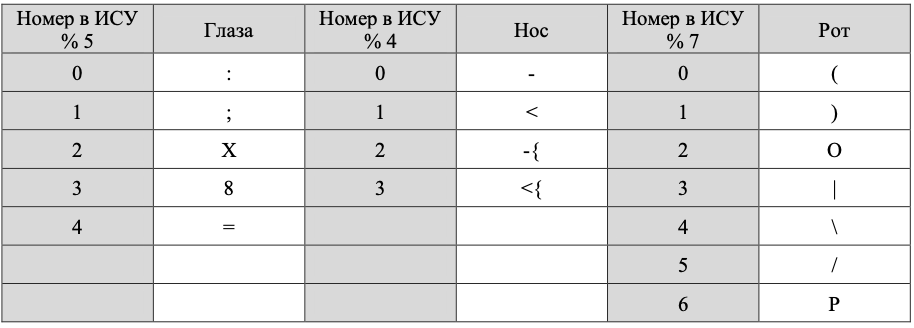
\includegraphics[]{images/no1.png}
\newline Мой вариант: 8<(
\paragraph{Код}
\hfill \break
\FloatBarrier
\lstloadlanguages{Python}
\definecolor{mygray}{RGB}{120,120,120}
\lstset{
inputencoding=utf8x,
extendedchars =\true,
breaklines=true,
basicstyle=\ttfamily\fontsize{9pt}{9pt}\selectfont,
commentstyle=\color{mygray},
keywordstyle=\color{blue},
keepspaces=true,
showstringspaces=false}
\lstinputlisting[language=Python,numbers=left]{prog1/prog1.py}
\paragraph{Тест1}
\hfill \break
\lstinputlisting[]{prog1/ptest1.txt}
\begin{minipage}{0.4\textwidth}
    \textbf{Результат программы:}\\
    2
  \end{minipage}
  \hfill
  \begin{minipage}{0.5\textwidth}
    \textbf{Результат руками:}\\
    \textbackslash\{\textcolor{blue}{8<(}7X-{Oo<(:<(;<(X<(\textcolor{blue}{8<(}}=<(8<{/8<|8<\textbackslash8<P8<)}
    Ответ: 2
  \end{minipage}
\paragraph{Тест2}
\hfill \break

\includegraphics[scale=0.4]{prog1/pt2.png}
\hfill \break
\textbf{Результат программы:}\\
2\\
\textbf{Результат руками:}
\hfill \break

\includegraphics[scale=0.4]{prog1/pt2+.png}
\paragraph{Тест3}
\hfill \break
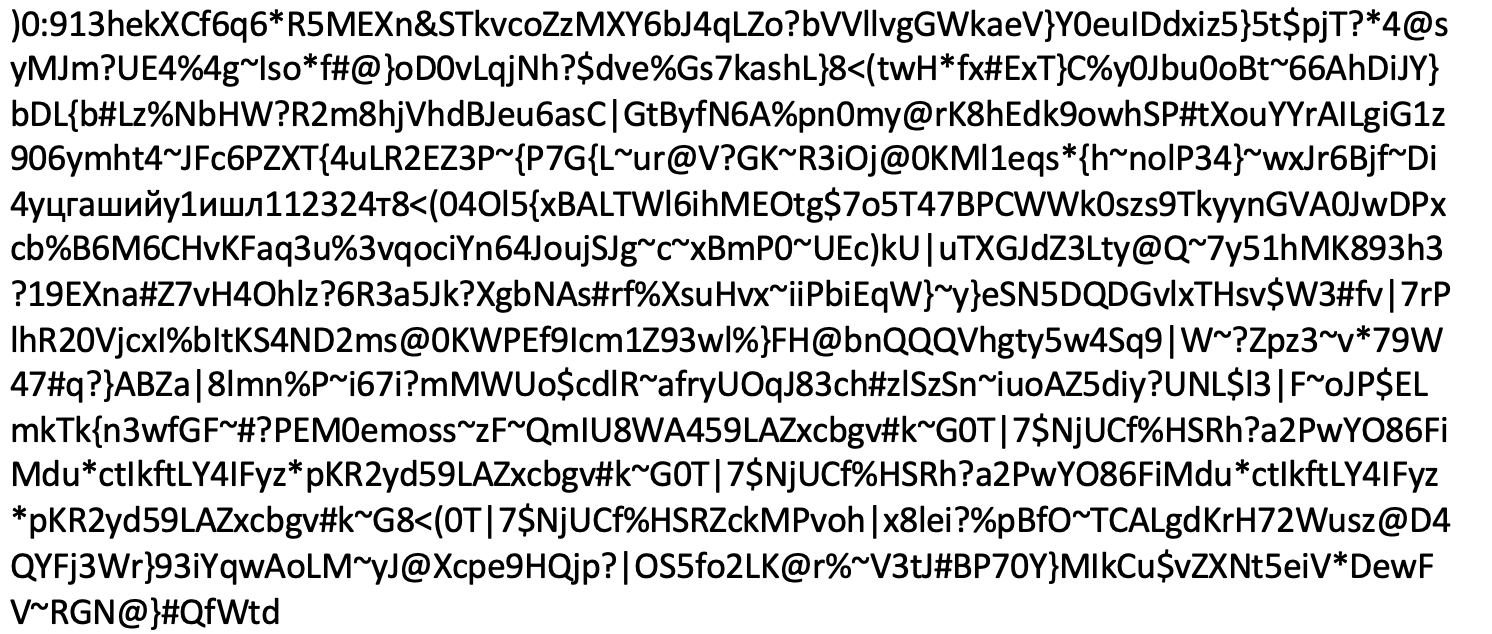
\includegraphics[scale=0.4]{prog1/pt3.png}
\hfill \break
\textbf{Результат программы:}\\
3\\
\textbf{Результат руками:}
\hfill \break
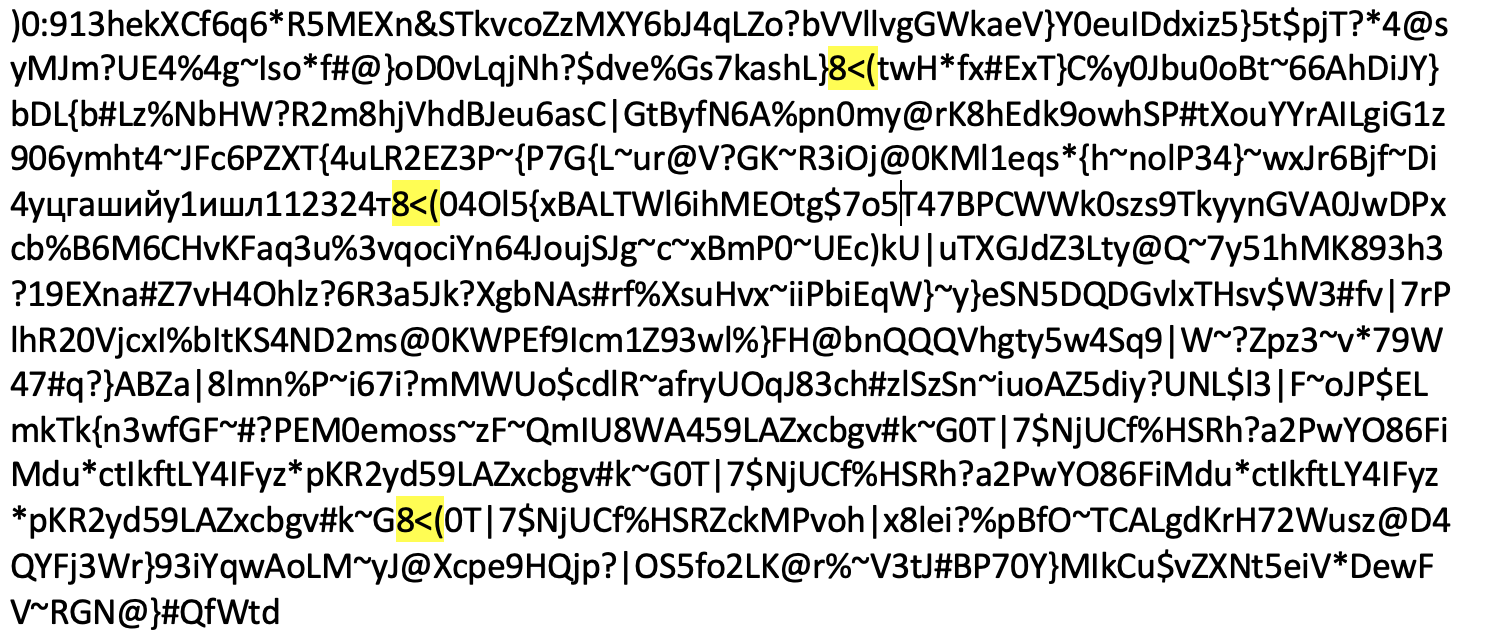
\includegraphics[scale=0.4]{prog1/pt3+.png}
\paragraph{Тест4}
\hfill \break
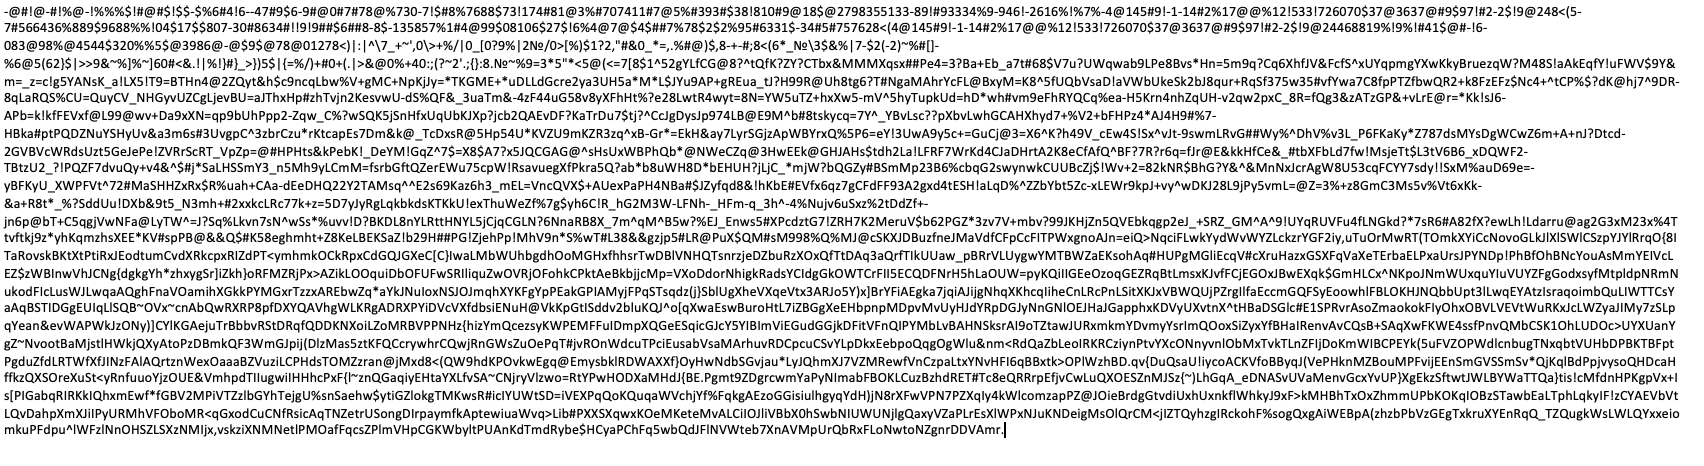
\includegraphics[scale=0.4]{prog1/pt4.png}
\hfill \break
\textbf{Результат программы:}\\
4\\
\textbf{Результат руками:}
\hfill \break
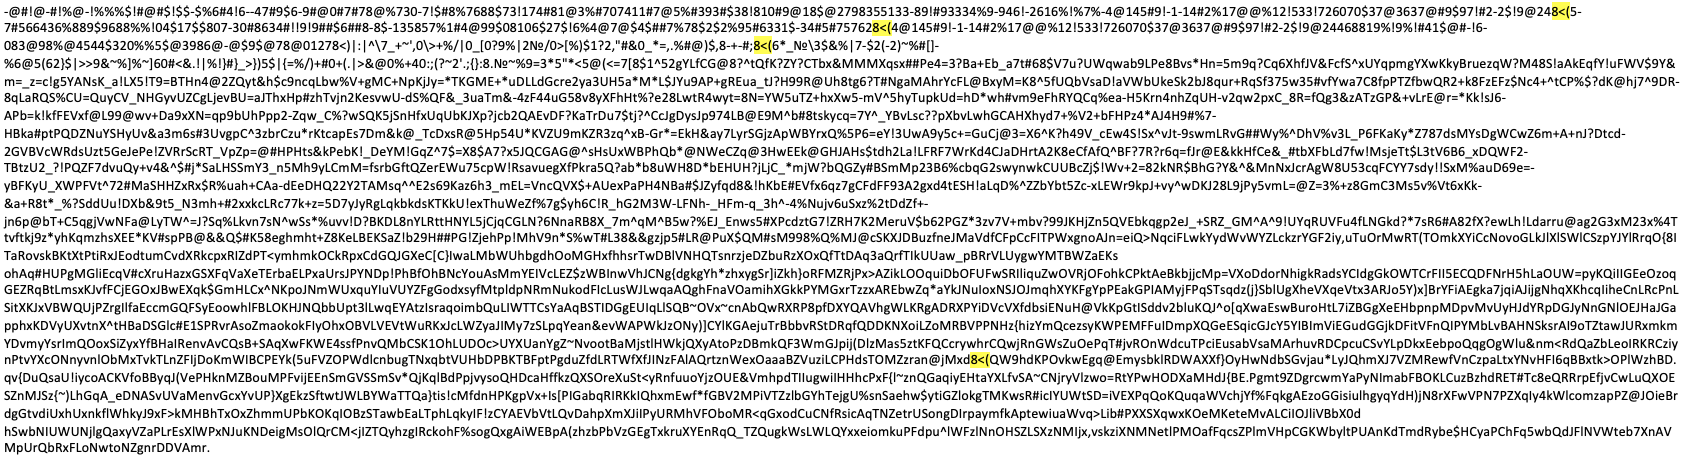
\includegraphics[scale=0.4]{prog1/pt4+.png}
\paragraph{Тест5}
\hfill \break

\includegraphics[scale=0.4]{prog1/pt5.png}
\hfill \break
\textbf{Результат программы:}\\
3\\
\textbf{Результат руками:}
\hfill \break
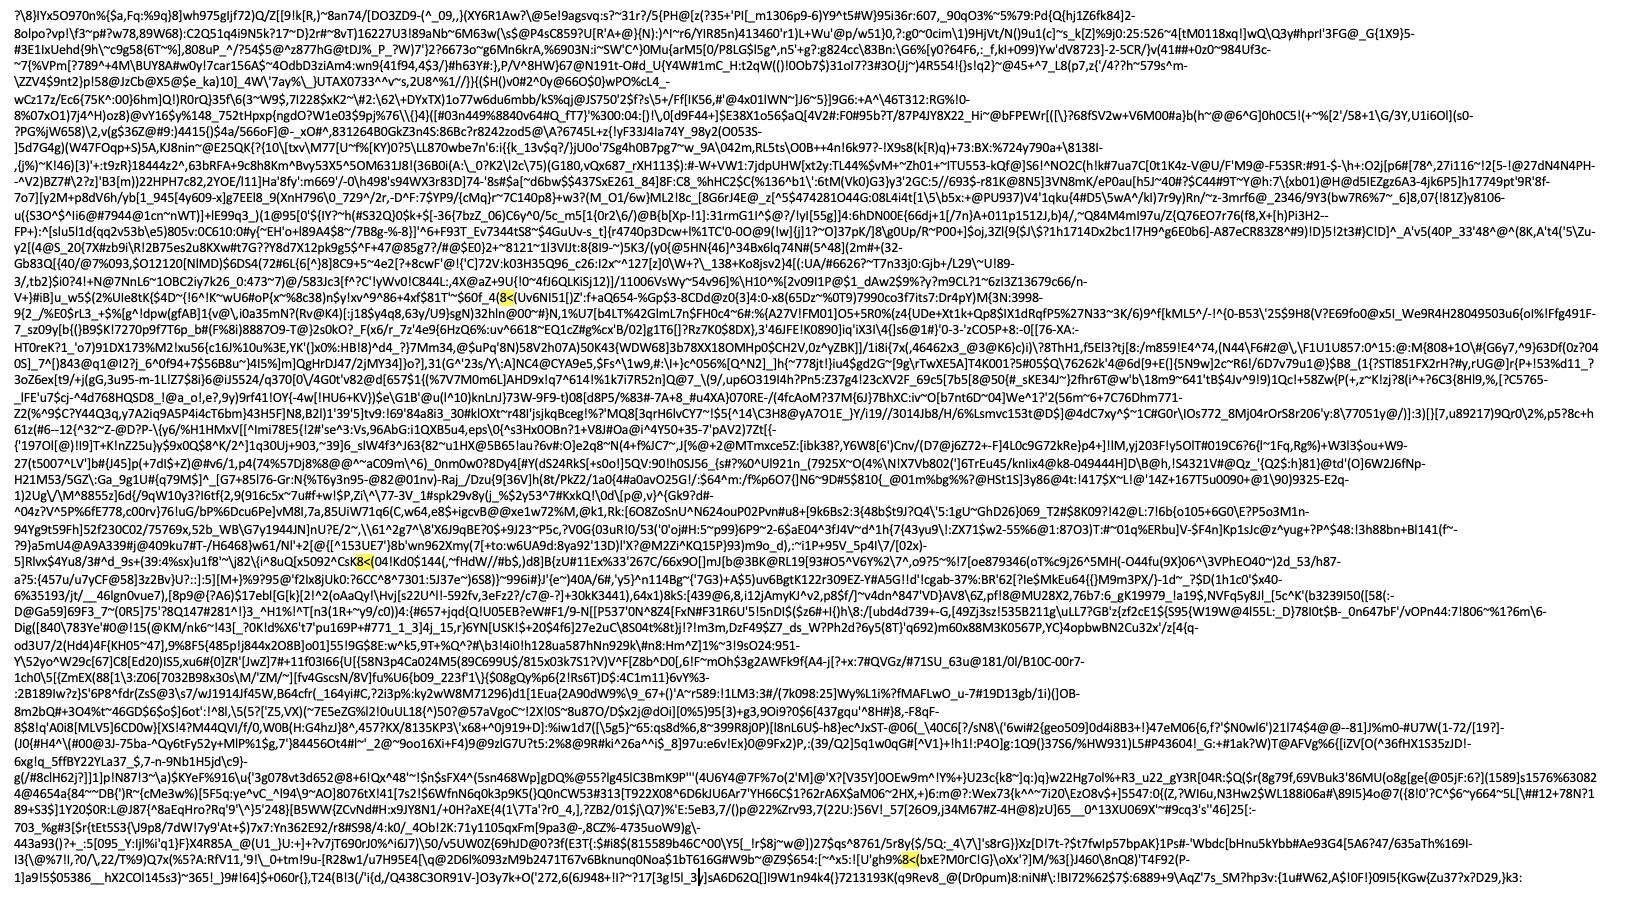
\includegraphics[scale=0.4]{prog1/pt5+.png}
\subsection{Доп. задание 1}
\paragraph{Текст задания:}
\hfill \break
1) Реализуйте программный продукт на языке Python, используя регулярные выражения по варианту, представленному в таблице.\\
2) Для своей программы придумайте минимум 5 тестов. Каждый тест является отдельной сущностью, передаваемой регулярному выражению для обработки. Для каждого теста необходимо самостоятельно (без использования регулярных выражений) найти правильный ответ. После чего сравнить ответ, выданный программой, и полученный самостоятельно.
Пример тестов приведён в таблице.
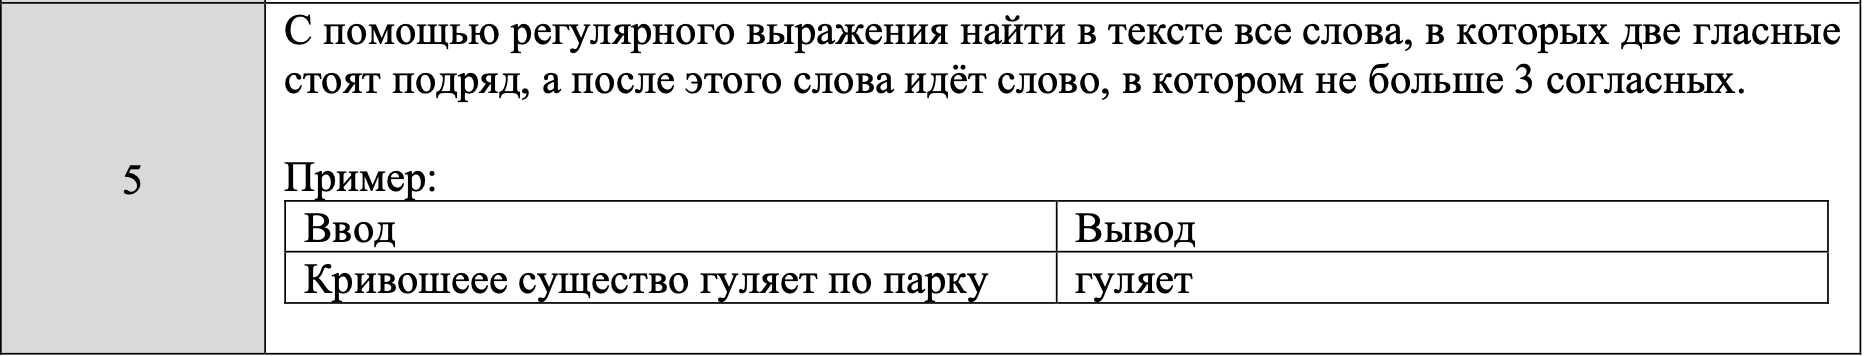
\includegraphics[scale=0.5]{images/no2.png}
\paragraph{Код}
\hfill \break
\FloatBarrier
\verbatiminput{prog2/prog2.py}
\paragraph{Тест 1}
\begin{verbatim}
  Кривошеее существо гуляет по парку еепрок роо гуляет попр кривошее по парку
\end{verbatim}
\textbf{Результат программы:}\\
гуляет еепрок роо гуляет кривошее\\
\textbf{Результат руками:}
\newline Кривошеее существо \textcolor{blue}{гуляет} по парку \textcolor{blue}{еепрок} \textcolor{blue}{роо} \textcolor{blue}{гуляет} попр \textcolor{blue}{кривошее} по парку
\paragraph{Тест 2}
\hfill \break
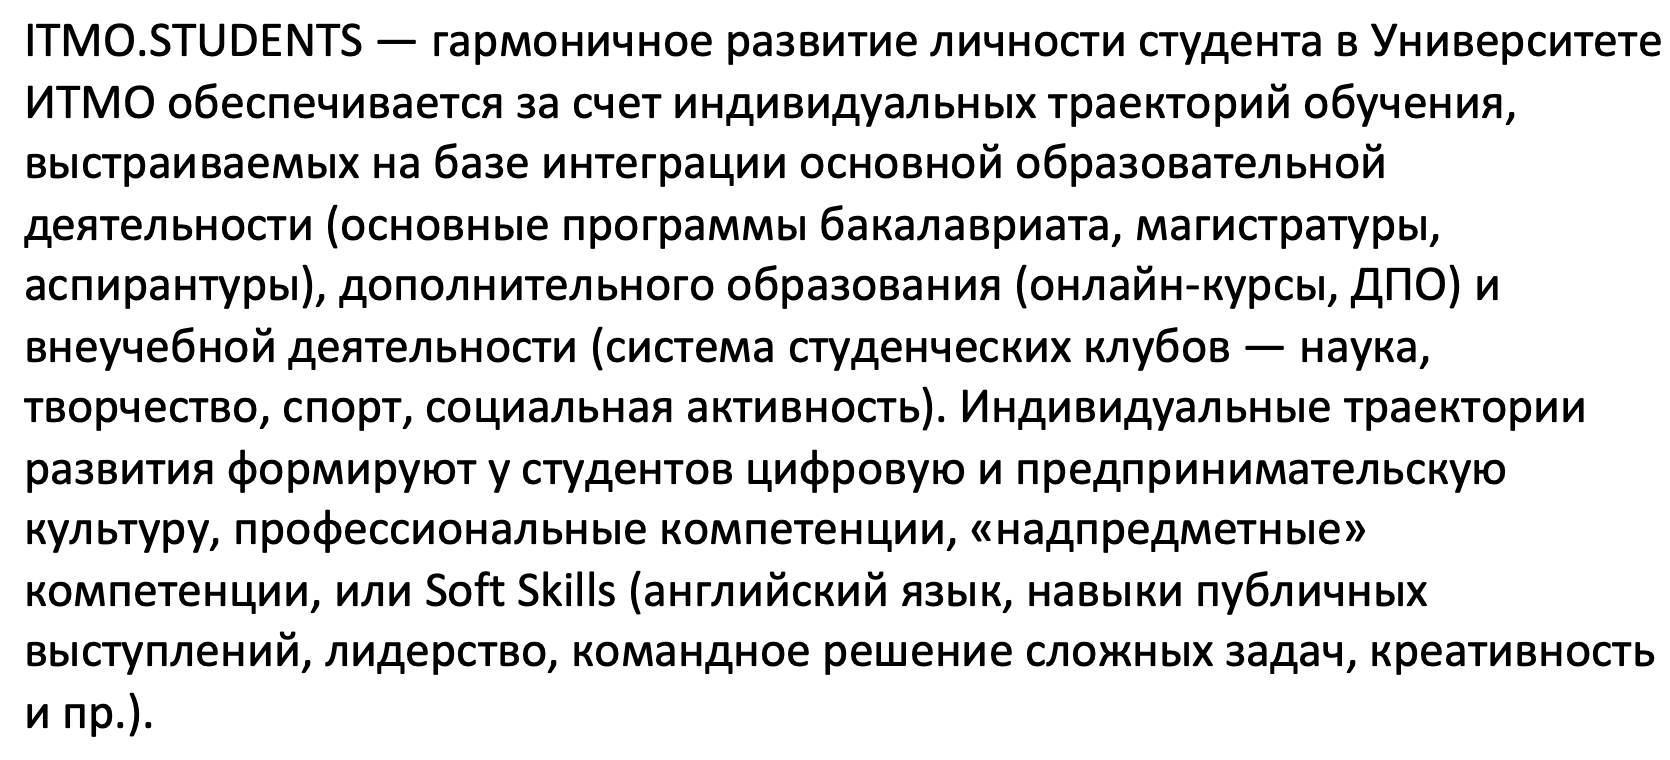
\includegraphics[scale=0.4]{prog2/p2.png}\\
\textbf{Результат программы:}\\
обеспечивается траекторий выстраиваемых командное\\
\textbf{Результат руками:}\\
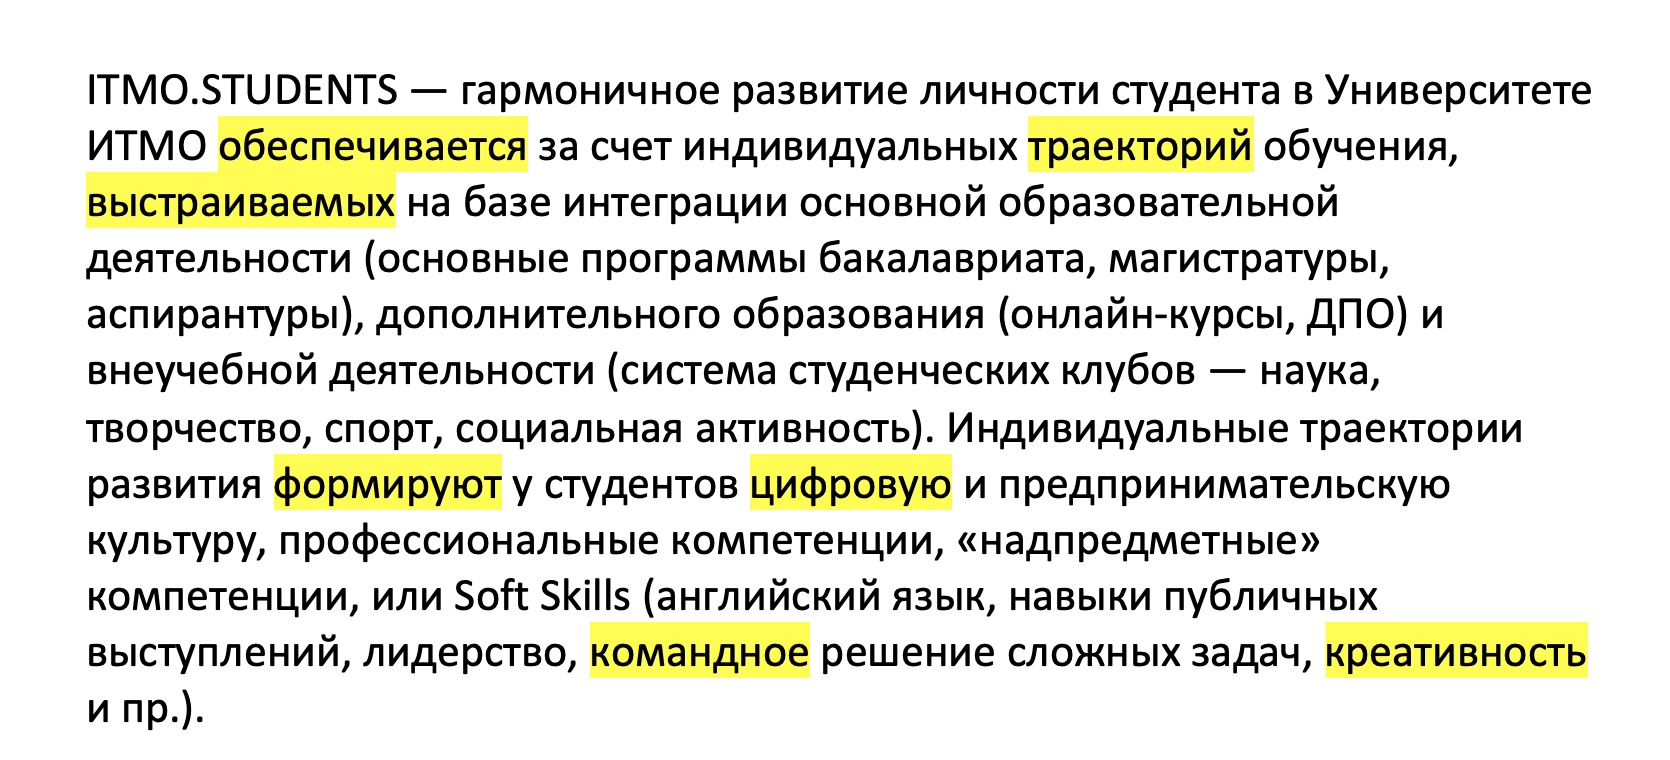
\includegraphics[scale=0.4]{prog2/p2+.png}\\
\paragraph{Тест 3}
\hfill \break

\includegraphics[scale=0.4]{prog2/p3.png}\\
\textbf{Результат программы:}\\
НИУ Функции науки Минобрнауки Минобрнауки науки Минобрнауки Минобрнауки\\
\textbf{Результат руками:}\\
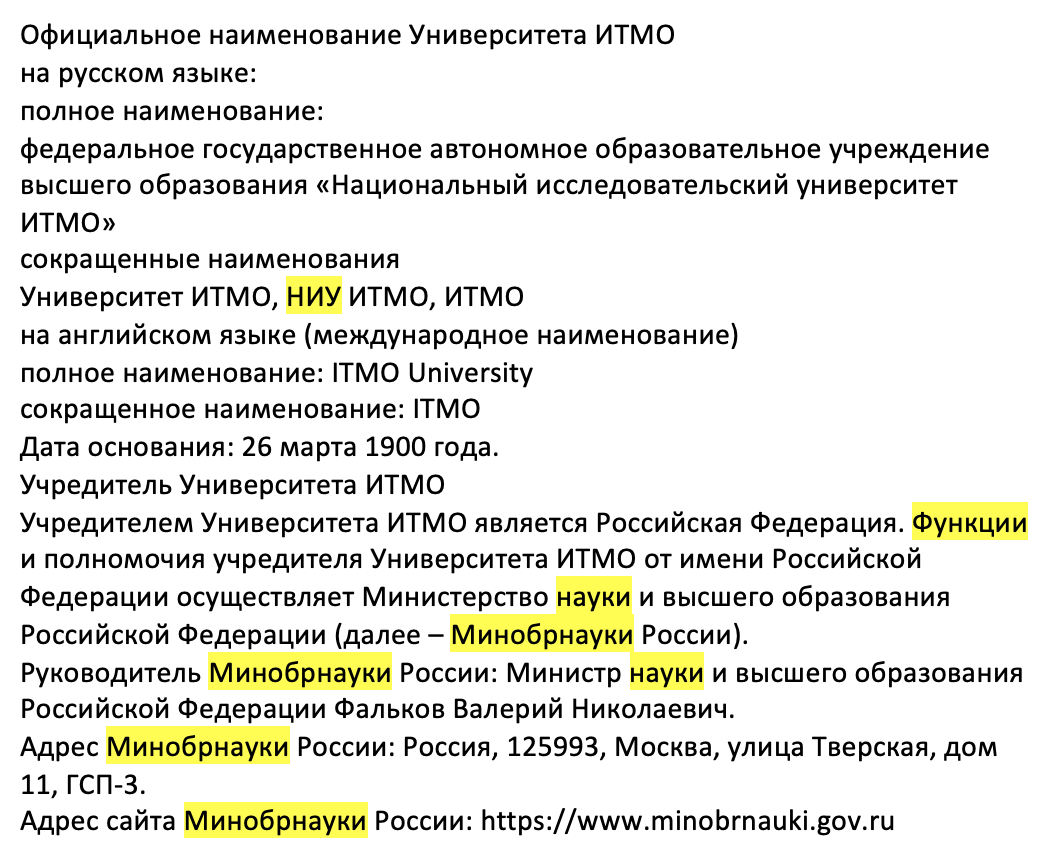
\includegraphics[scale=0.4]{prog2/p3+.png}\\
\paragraph{Тест 4}
\hfill \break
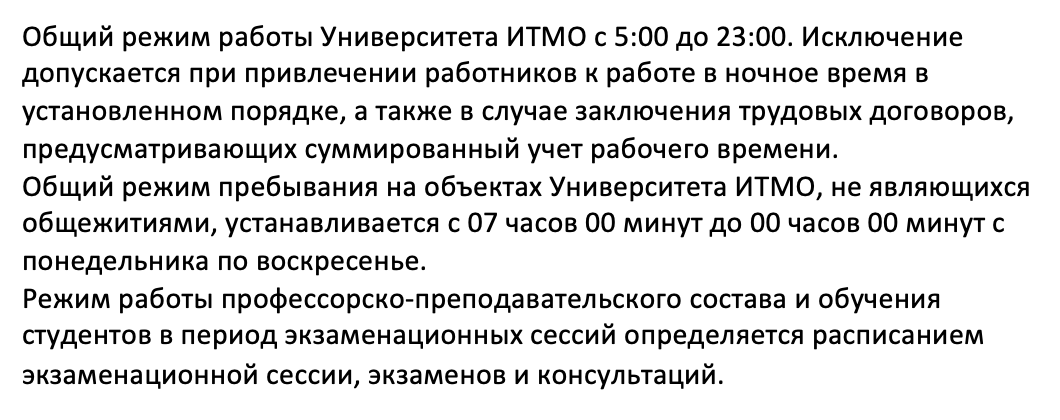
\includegraphics[scale=0.4]{prog2/p4.png}\\
\textbf{Результат программы:}\\
допускается ночное пребывания устанавливается экзаменационной\\
\textbf{Результат руками:}\\
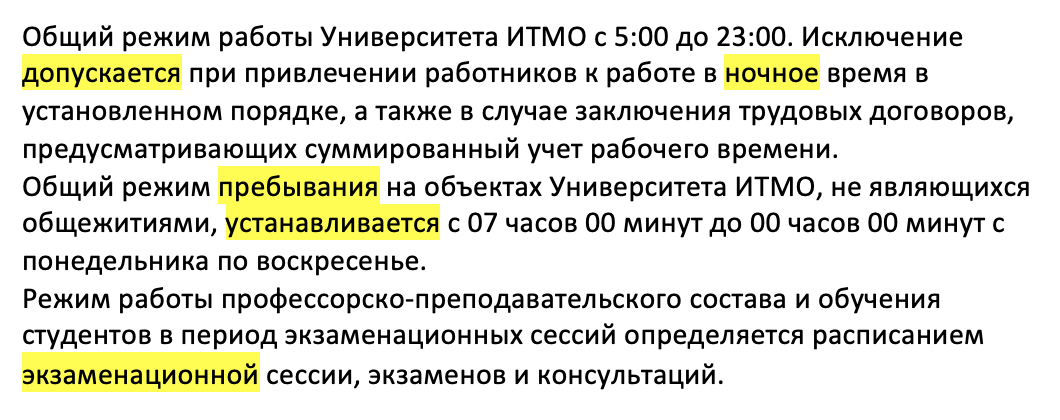
\includegraphics[scale=0.4]{prog2/p4+.png}\\
\paragraph{Тест 5}
\hfill \break
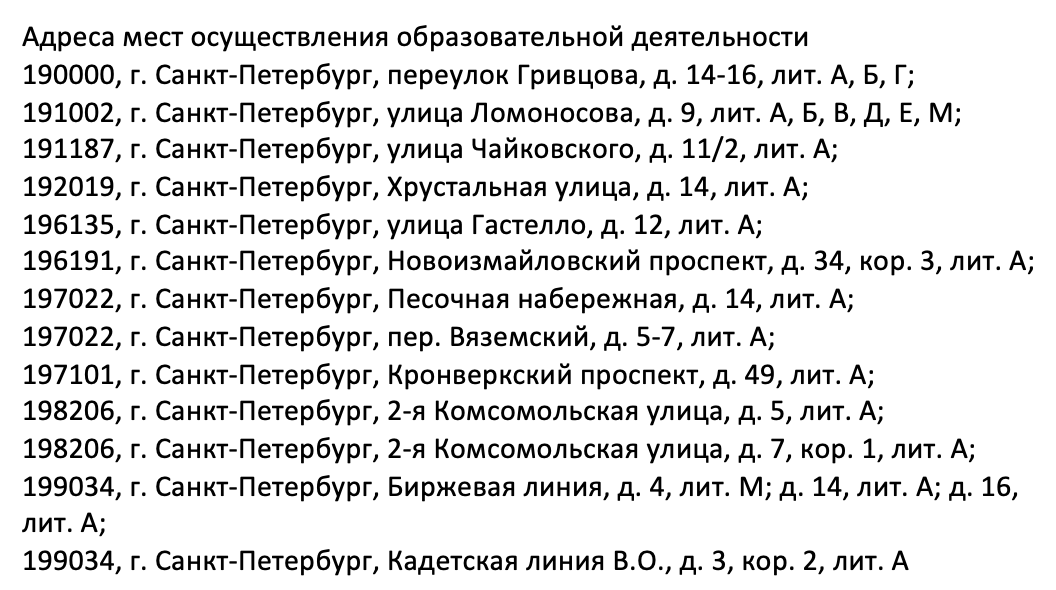
\includegraphics[scale=0.4]{prog2/p5.png}\\
\textbf{Результат программы:}\\
Хрустальная набережная Комсомольская Комсомольская Биржевая линия Кадетская линия\\
\textbf{Результат руками:}\\
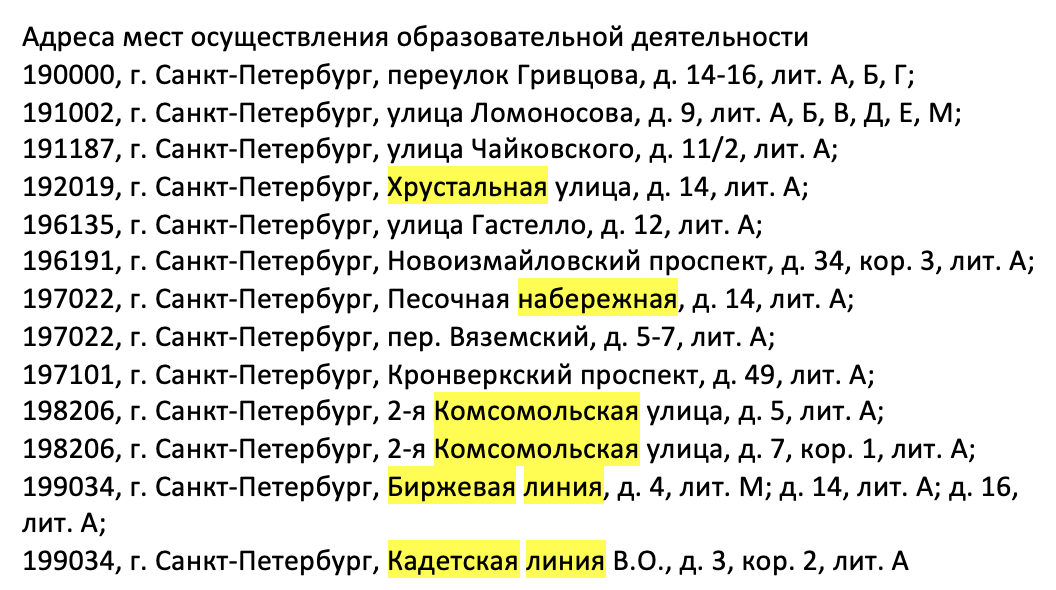
\includegraphics[scale=0.4]{prog2/p5+.png}\\
\subsection{Доп. задание 2}
\paragraph{Текст задания:}
\hfill \break
1) Реализуйте программный продукт на языке Python, используя регулярные выражения по варианту, представленному в таблице.\\
2) Для своей программы придумайте минимум 5 тестов.\\
3) Протестируйте свою программу на этих тестах.\\
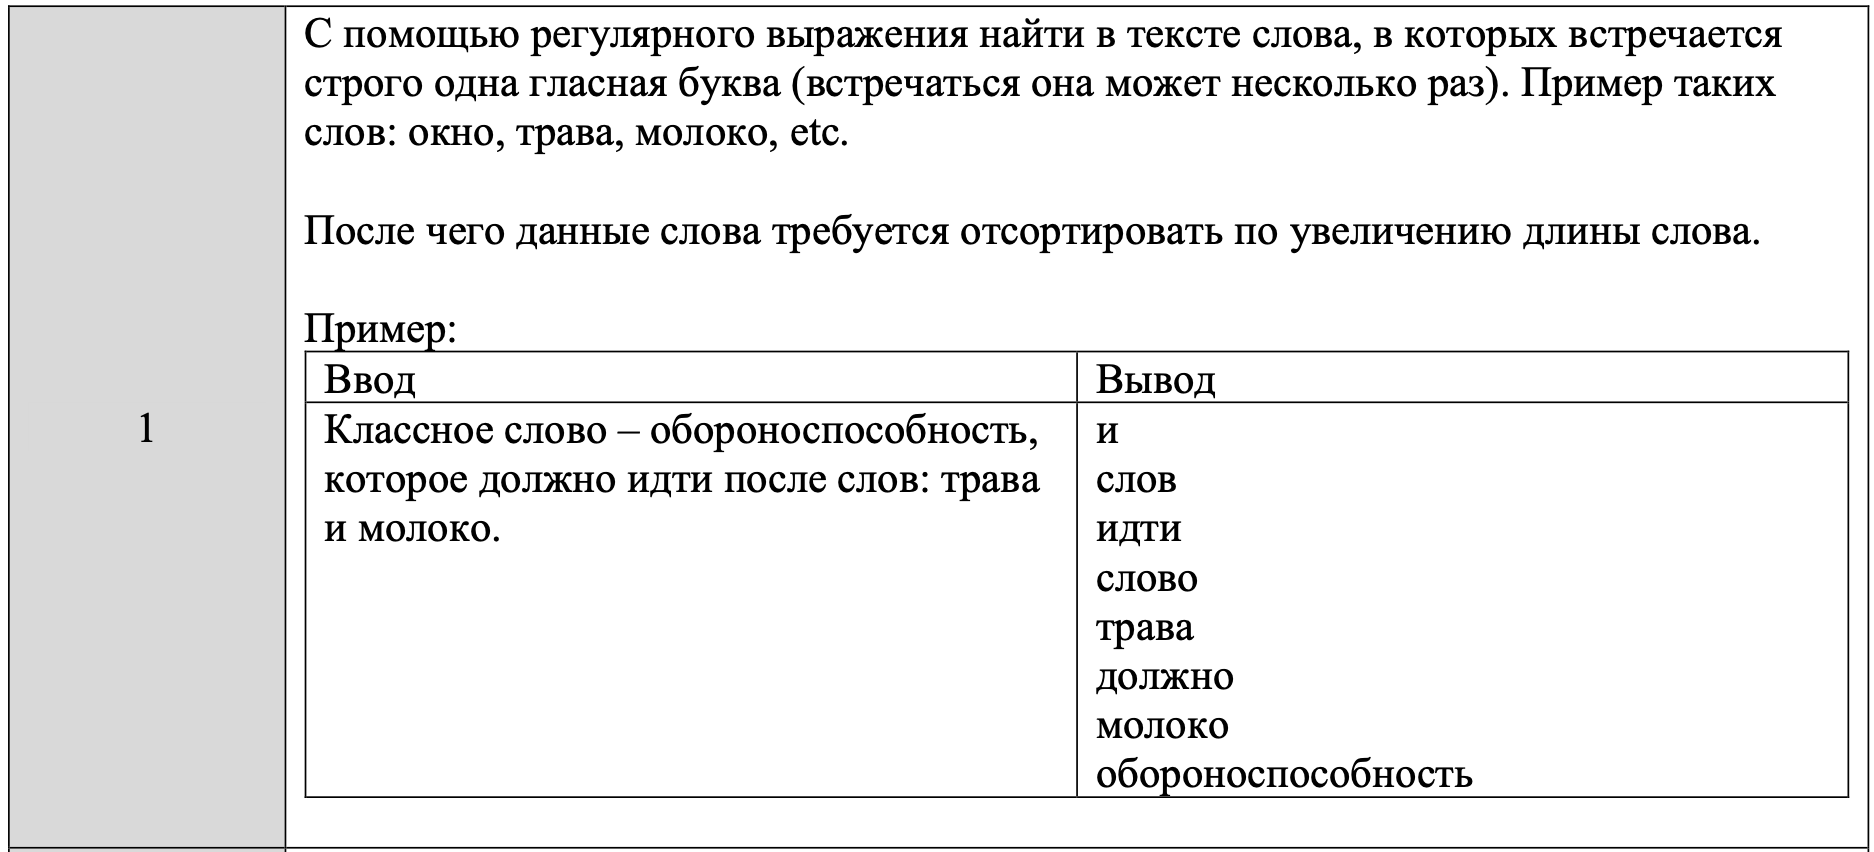
\includegraphics[scale=0.5]{images/no3.png}
\paragraph{Код}
\hfill \break
\FloatBarrier
\begingroup
    \fontsize{10pt}{12pt}\selectfont
    \verbatiminput{prog3/prog3.py}  
\endgroup
\hfill \break
\paragraph{Тест 1}
\hfill \break
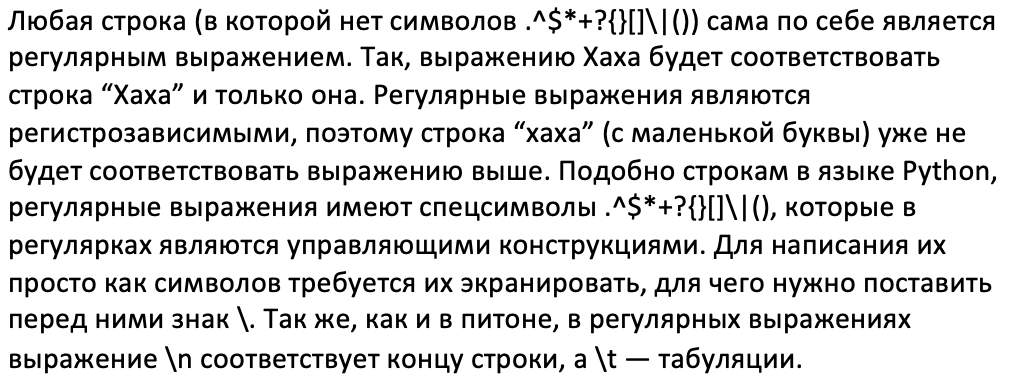
\includegraphics[scale=0.5]{prog3/p1.png}\\
\textbf{Результат программы:}\\
\begingroup
    \fontsize{10pt}{12pt}\selectfont
    \begin{verbatim}  
      и
      и
      а
      по
      не
      их
      их
      же
      нет
      Так
      Для
      как
      для
      Так
      как
      сама
      себе
      Хаха
      Хаха
      хаха
      ними
      знак
      перед
      только
      просто
      которой
      Подобно
    \end{verbatim}  
\endgroup
\paragraph{Тест 2}
\hfill \break
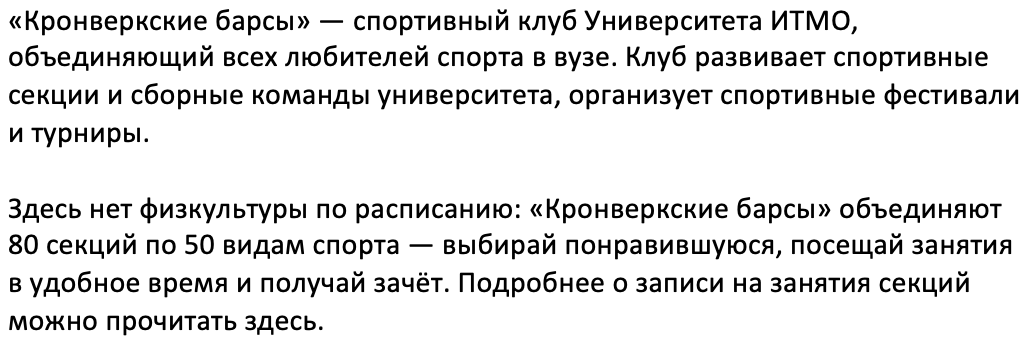
\includegraphics[scale=0.4]{prog3/p2.png}\\
\textbf{Результат программы:}\\
\begingroup
    \fontsize{10pt}{12pt}\selectfont
    \begin{verbatim}  
      и
      и
      и
      о
      по
      по
      на
      нет
      клуб
      всех
      Клуб
      Здесь
      можно
      здесь
    \end{verbatim}  
\endgroup

\paragraph{Тест 3}
\hfill \break
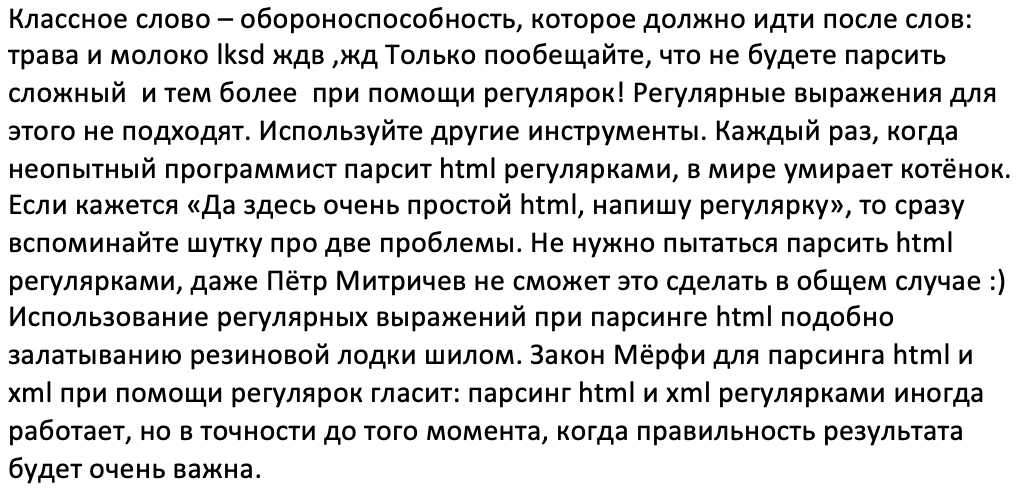
\includegraphics[scale=0.4]{prog3/p3.png}\\
\textbf{Результат программы:}\\
\begingroup
    \fontsize{10pt}{12pt}\selectfont
    \begin{verbatim}  
и
и
и
и
не
не
Да
то
Не
не
но
до
что
тем
при
для
раз
про
две
при
для
при
идти
слов
Пётр
того
слово
трава
здесь
шутку
важна
должно
молоко
Только
простой
подобно
обороноспособность
    \end{verbatim}  
\endgroup
\paragraph{Тест 4}
\hfill \break
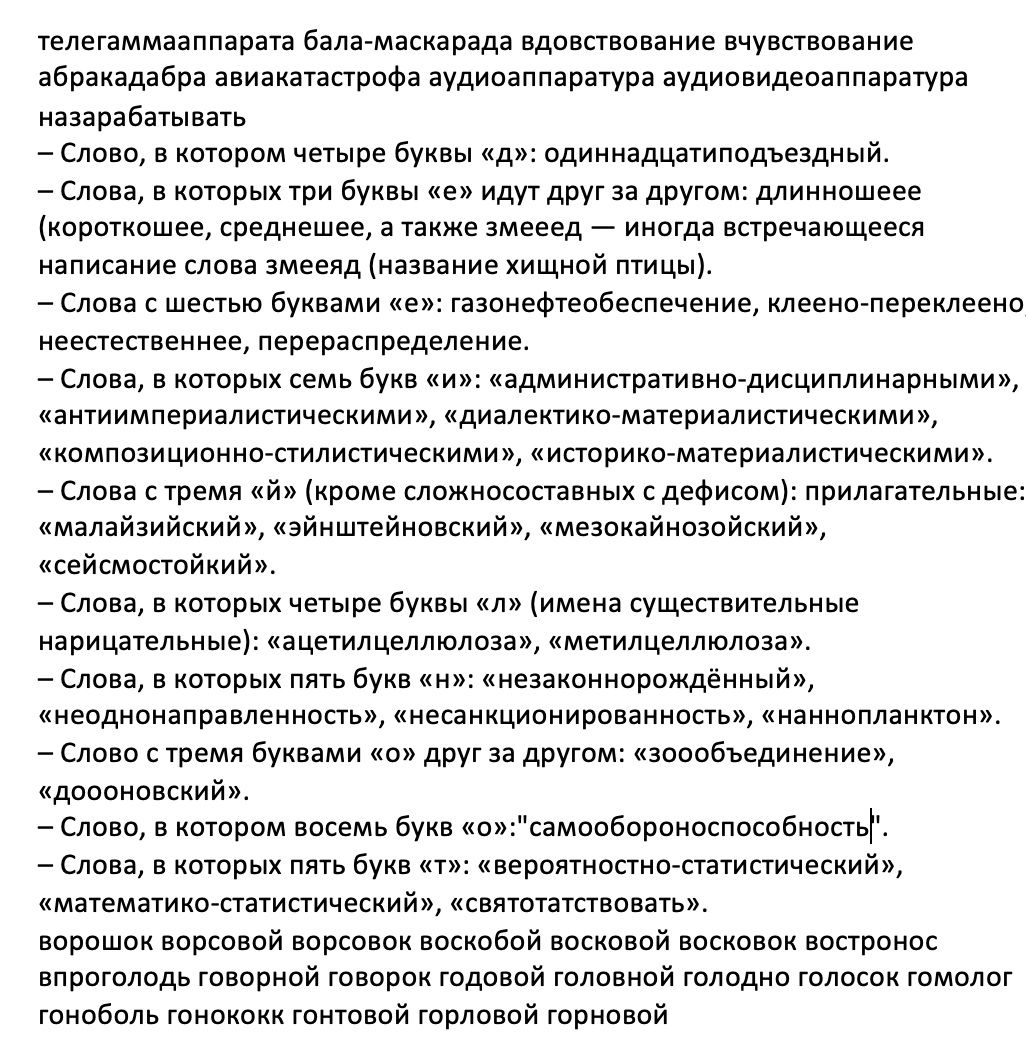
\includegraphics[scale=0.4]{prog3/p4.png}\\
\textbf{Результат программы:}\\
\begingroup
    \fontsize{10pt}{12pt}\selectfont
    \begin{verbatim}  
      е
      а
      е
      и
      о
      за
      за
      три
      друг
      семь
      букв
      пять
      букв
      друг
      букв
      пять
      букв
      Слово
      Слово
      Слово
      змееед
      котором
      котором
      ворошок
      говорок
      годовой
      голосок
      гомолог
      ворсовой
      ворсовок
      воскобой
      восковой
      восковок
      говорной
      головной
      голодной
      гоноболь
      гонококк
      гонтовой
      горловой
      горновой
      среднешее
      востронос
      впроголодь
      абракадабра
      баламаскарада
      неестественнее
    \end{verbatim}  
\endgroup

\paragraph{Тест 5}
\hfill \break
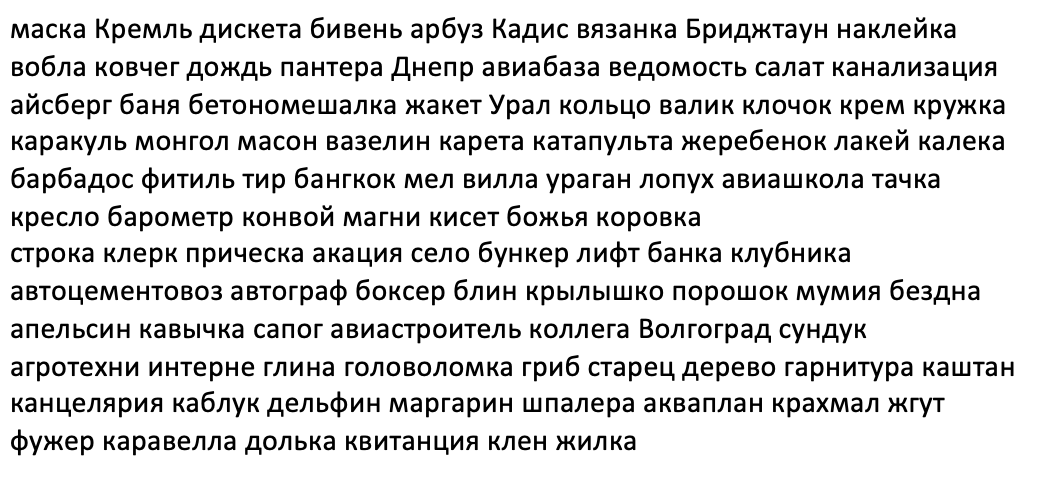
\includegraphics[scale=0.4]{prog3/p5.png}\\
\textbf{Результат программы:}\\
\begingroup
    \fontsize{10pt}{12pt}\selectfont
    \begin{verbatim}  
      тир
      мел
      крем
      лифт
      блин
      гриб
      жгут
      клен
      маска
      дождь
      Днепр
      салат
      тачка
      клерк
      банка
      Кремль
      кольцо
      клочок
      монгол
      фитиль
      конвой
      сундук
      каштан
      порошок
      крахмал
      акваплан
    \end{verbatim}  
\endgroup
\section{Вывод:}
В этой лабораторной работе я познакомился языком регулярных выражений. Научился работать с регулярными выражениями в языке Python.
\end{flushleft}
\begin{thebibliography}{2}
\addcontentsline{toc}{section}{\bibname}
\bibitem {1}
\href{https://habr.com/ru/post/545150/}{Регулярные выражения (regexp) — основы} --- @Molechka
\bibitem {2}
\href{https://habr.com/ru/post/349860/}{Регулярные выражения в Python от простого к сложному. Подробности, примеры, картинки, упражнения} --- Сергей Шашков
\end{thebibliography}
\end{document}